\documentclass{zkdl-presentation-template}

\usepackage{graphicx}

\title[Sum-Check Toolkit]{\textbf{Sum-Check Toolkit}}
\author{Distributed Lab}
\date{July 17, 2024}
\homepage{zkdl-camp.github.io}
\github{ZKDL-Camp}

\begin{document}
    \frame {
        \tikz [remember picture,overlay]
        \node at
            ([yshift=1.5cm,xshift=-1.5cm]current page.south east) 
            %or: (current page.center)
            {
\includegraphics[width=60pt]{images/logo.png}};
        \titlepage
    }

	\section{Sum-Check-based Protocol for Grand Products}

    \begin{frame}{Grand Product Relation}
        \begin{equation*}
        \mathcal{R}_{GP} = \big\{ (p \in \mathbb{F}, \mathbf{v} \in \mathbb{F}^m)\colon p = \prod_{i=0}^m v_i \big\} \label{grand-product-relation}
        \end{equation*}
        Assume that $m$ is a power of $2$.

        \pause
        
        Let $\widetilde{v}$ be an MLE of $\mathbf{v}$, by viewing $\mathbf{v}$ as a 
        function mapping $\{0,1\}^{\log m} \rightarrow \mathbb{F}$.
    \end{frame}

    \begin{frame}{Main Lemma}
        \begin{lemma}
        A scalar $p$ and a vector $\mathbf{v}$ satisfies the relation $\mathcal{R}_{GP}$ if and only if there exists a 
        multilinear polynomial $f$ in $\log m + 1$ variables such that $f(1,\dots,1, 0) = p$ and $\forall x \in \{0,1\}^{\log m}$
        the following hold:
        \begin{gather*}
        f(0, x) = v(x)\\
        f(1,x) = f(x, 0) \cdot f(x, 1)
        \end{gather*}
        Such polynomial $f$ has the following construction: \begin{itemize}
            \item $f(1,\dots,1) = 0$
            \item For all $\ell \in [\log m]$ and $x \in \{0,1\}^{\log m - \ell}$: \\ 
            \vspace{-0.8em}
            \begin{equation*}
                f(1^\ell, 0, x) = \prod_{y \in \{0,1\}^\ell}v(x,y)
            \end{equation*}
        \end{itemize}
        \end{lemma}
    \end{frame}

    \begin{frame}
        \begin{example}
            Let $m=4$ ($\log m=2$), $\mathbf{v} = \{1, 2, 3, 4\}$, consequently $p = 1\times2\times3\times4=24$, then:
            \vspace{-5px}
            \pause
            \begin{align*}
            v(x_1, x_2)& = 1 + 2x_1 + x_2\\
            v(x_1,x_2)&: \quad v(0,0)=1,\; v(0,1)=2,\; v(1,0)=3,\; v(1,1)=4.
            \vspace{-5px}
            \end{align*}
            \pause
            Now, we define $f$ as follows:
            \vspace{-5px}
            \begin{equation*}
                f(0,0,0)= 1,\; f(0,0,1)=2,\; f(0,1,0)=3,\; f(0,1,1)=4,
                \vspace{-5px}
            \end{equation*}
            \pause
            and:
            \vspace{-10px}
            \begin{align*}
            f(1,0,0)&= f(0,0,0) \times f(0,0,1) = 1 \times 2 = 2,\\ 
            f(1,0,1)&= f(0,1,1) \times f(0,1,1) = 3 \times 4 = 12,\\ 
            f(1,1,0)&= f(1,0,0) \times f(1,0,1) = 2 \times 12 = 24 = p,\\ 
            f(1,1,1)&= 0.
            \vspace{-5px}
            \end{align*}
        \end{example}
    \end{frame}

    \begin{frame}
        \begin{example}
            \begin{center}
                \scalebox{1.0}{
                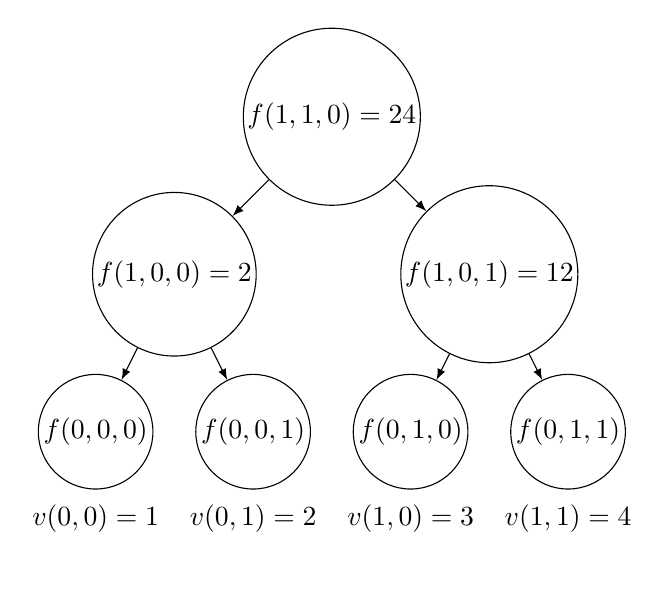
\begin{tikzpicture}[
                    level 1/.style={level distance=2cm, sibling distance=4cm},
                    level 2/.style={level distance=2cm, sibling distance=2cm},
                    level 3/.style={level distance=1.1cm, sibling distance=2cm, edge from parent/.style={draw=none},},
                    edge from parent/.style={draw, -latex},
                    every node/.style={circle,draw,inner sep=1pt}
                ]
                \node {$f(1,1,0)=24$}
                    child {
                        node {$f(1,0,0)=2$}
                        child { node {$f(0,0,0)$}
                            child { node[draw=none] {$\displaystyle v(0,0)=1$} }
                        }
                        child { node {$f(0,0,1)$}
                            child { node[draw=none] {$\displaystyle v(0,1)=2$} }
                        }
                    }
                    child {
                        node {$f(1,0,1)=12$}
                        child { node {$f(0,1,0)$}
                            child { node[draw=none] {$\displaystyle v(1,0)=3$} }
                        }
                        child { node {$f(0,1,1)$}
                            child { node[draw=none] {$\displaystyle v(1,1)=4$} }
                        }
                    };
                \end{tikzpicture}
                }
            \end{center}
            \vspace{-15px}
        \end{example}
    \end{frame}

    \begin{frame}{Where Is Sum-Check?}
        \centering
        % Adjust width or height as needed:
        
\includegraphics[width=1\linewidth]{./images/lecture_17/where-is-everyone.png}
        \label{fig:meme}
    \end{frame}

    \begin{frame}{Zero-Check}
        \begin{equation*}
            \forall x \in \{0,1\}^{\log m}\colon f(1,x) = f(x, 0) \cdot f(x, 1)
        \end{equation*}
        \pause
        \vspace{-10px}
        \begin{equation*}
            \forall x \in \{0,1\}^{\log m}\colon f(1,x) - f(x, 0) \cdot f(x, 1) = 0
        \end{equation*}
        \pause
        One can use the sum-check protocol to prove the evaluation of $g$ that is referred to a MLE of $f(1,x) - f(x, 0) \cdot f(x, 1)$:
        \begin{equation*}
            g(t) = \sum_{x \in \{0,1\}^{\log m}} \widetilde{\text{eq}}(t,x) \cdot (f(1,x) - f(x, 0) \cdot f(x, 1))
        \end{equation*}
        By the Schwartz–Zippel lemma, for random $\tau \in \mathbb{F}^{\log m}$,
        $g(\tau) = 0$ if and only if $g = 0$, except for a soundness error of $\frac{\log m}{|\mathbb{F}|}$.
    \end{frame}

    \begin{frame}
        Thus, to prove the existence of $f$ and hence the grand product relationship, it suffices
        to prove, for some verifier selected random $\tau, \gamma \in \mathbb{F}^\ell$, that:
        \begin{gather}
        \label{eq:grands0}
            0 = \sum_{x \in \{0,1\}^{\log m}} \widetilde{\text{eq}}(x, \tau) \cdot (f(1,x) - f(x, 0) \cdot f(x, 1))\\
        \label{eq:grands1}
            f(0, \gamma) = \widetilde{v}(\gamma)\\
        \label{eq:grands2}
            f(1,\dots,1, 0) = p
        \end{gather}
    \end{frame}

    \begin{frame}
        \begin{algorithm}[H]
            \caption{Sum-Check-based Protocol for Grand Products}\label{alg:sum_check_grand_product}
            \DontPrintSemicolon
            \SetAlgoLined

            \textbf{$\mathcal P$:}
            Compute polynomials 
            $v\in\mathbb{F}^{\log m}[x]$, 
            $f\in\mathbb{F}^{\log m+1}[x]$ 
            such that
            \vspace{-1em}
            \begin{equation*}
                \vspace{-1.6em}
                p = \prod_{x\in\{0,1\}^{\log m}} v(x)
                \quad\text{and}\quad
                f, v \text{ satisfy }(\ref{eq:grands0}),\,(\ref{eq:grands1}),\,(\ref{eq:grands2}).
                \vspace{-5px}
            \end{equation*}\;

            \textbf{$\mathcal P$:}
            $C_f \leftarrow \textsc{Commit}(f)$;
            $C_v \leftarrow \textsc{Commit}(v)$;
            send $C_f, C_v$ to $\mathcal V$.\;

            \textbf{$\mathcal V$:}
            Choose random $\tau,\gamma\in\mathbb{F}^{\log m}$ and send them to $\mathcal P$.\;

            \textbf{$\mathcal P$:}
            Compute $g(x)\;=\;\widetilde{\mathrm{eq}}(x,\tau)\,\bigl(f(1,x)-f(x,0)\,f(x,1)\bigr).$

            \textbf{$\mathcal P$ \& $\mathcal V$:}
            Run \textsc{SumCheckProtocol}($0,\;g,\;C_f$)

            \textbf{$\mathcal V$:}
            $a \leftarrow \textsc{Query}(C_f,(0,\gamma)), \;$ $v(\gamma)\leftarrow \textsc{Query}(C_v,\gamma)$.\;
            \If{$a \neq v(\gamma)$}{
                \textbf{$\mathcal V$ rejects}.\;
            }

            \textbf{$\mathcal V$:}
            $r \leftarrow \textsc{Query}(C_f,(1,\dots,1,0))$.\;
            \If{$r \neq p$}{
                \textbf{$\mathcal V$ rejects}.\;
            }
        \end{algorithm}
    \end{frame}

    \section{Randomized Permutation Check}

    \begin{frame}
        The goal is to verify, with high probability, whether two sequences of tuples
        are permutations of each other, without performing a full sort or pairwise comparison.

        \pause
        \begin{equation*}
        A = \{(1,2,3),\,(4,0,6)\}, \quad
        B = \{(4,0,6),\,(1,2,3)\}.
        \end{equation*}
        \textit{The naive approach would be to sort both sequences and then compare them.}
    \end{frame}

    \begin{frame}{Reed-Solomon Fingerprinting}
        \begin{definition}[Reed-Solomon Fingerprinting]
            Let $\mathbf{a} \in \mathbb{F}^{n}$, then for a random $\gamma \in \mathbb{F}$, the Reed-Solomon 
            fingerprinting of $\mathbf{a}$ is defined as:
            \begin{equation*}
                h_{\gamma}(\mathbf{a}) = \sum_{i \in n} a_i \cdot \gamma^i.
            \end{equation*}

            \pause
            $h_{\gamma}(\mathbf{a})$ uniquely identifies the sequence $\mathbf{a}$ with high probability,
            i.e., \\let $\mathbf{b} \in F^n$ and $\mathbf{a} \neq \mathbf{b}$, then, according to the Schwartz-Zippel lemma:
            \begin{equation*}
                \Pr[h_{\gamma}(\mathbf{a}) = h_{\gamma}(\mathbf{b})] \leq \frac{n}{|\mathbb{F}|}.
            \end{equation*}
        \end{definition}
    \end{frame}

    \begin{frame}{Reed-Solomon Fingerprinting}
        \begin{example}
            Consider all operations in $\mathbb{F}_7$, and set $n=3$, $\gamma=3$.  
            Let
            \begin{equation*}
                \mathbf{a} = (1,2,3), \quad \mathbf{b} = (4,0,6).
            \end{equation*}
            Then
            \begin{align*}
                h_{\gamma}(1,2,3) &=1\cdot3^0 + 2\cdot3^1 + 3\cdot3^2 =1 + 6 + 6 =13 \equiv 6,\\
                h_{\gamma}(4,0,6) &=4\cdot1 + 0\cdot3 + 6\cdot2 =4 + 0 + 12 =16 \equiv 2.
            \end{align*}
        \end{example}
    \end{frame}

    \begin{frame}{Randomized Permutation Check}
        \begin{definition}[Randomized Permutation Check]
            Let $A$ and $B$ be two multisets of tuples in $\mathbb{F}^n$. Define
            \begin{equation*}
                \mathcal{H}_{\tau,\gamma}(X)\;=\;\prod_{x \in X}\bigl(h_{\gamma}(x)-\tau\bigr).
            \end{equation*}
            \pause
            Then comparing $\mathcal{H}_{\tau,\gamma}(A)$ and $\mathcal{H}_{\tau,\gamma}(B)$ yields a
            randomized test for whether $A$ and $B$ are permutations of one another.\pause Concretely:
            \begin{itemize}
                \item (Completeness) If $A=B$ (as multisets), then  
                    \vspace{-5px}
                    \begin{equation*}
                        \mathcal{H}_{\tau,\gamma}(A)=\mathcal{H}_{\tau,\gamma}(B)
                        \vspace{-5px}
                    \end{equation*}
                    with probability 1 over uniform $\tau,\gamma\in\mathbb{F}$.
                \item (Soundness) If $A\neq B$, then
                    \vspace{-5px}
                    \begin{equation*}
                        \Pr\left[\,\mathcal{H}_{\tau,\gamma}(A)=\mathcal{H}_{\tau,\gamma}(B)\right]\;\le\; \frac{\max(|A|,|B|)}{|\mathbb{F}|}.
                    \end{equation*}
            \end{itemize}
        \end{definition}
    \end{frame}

    \begin{frame}
        \begin{example}
            Consider all operations in $\mathbb{F}_7$, set $n=3$, $\tau=5$, and $\gamma=3$.\\
            Let $A = \{(1,2,3),\,(4,0,6)\}, \quad B = \{(4,0,6),\,(1,2,3)\}.$
            
            \pause
            \vspace{5px}
            First compute the Reed–Solomon fingerprints modulo 7:
            \vspace{-7px}
            \begin{align*}
                h_{\gamma}(1,2,3) &=1\cdot3^0 + 2\cdot3^1 + 3\cdot3^2 =1 + 6 + 6 =13 \equiv 6,\\
                h_{\gamma}(4,0,6) &=4\cdot1 + 0\cdot3 + 6\cdot2 =4 + 0 + 12 =16 \equiv 2. \\[-23pt]
            \end{align*}
            \pause
            Now form the shifted products:
            \vspace{-7px}
            \begin{align*}
                \mathcal{H}_{\tau,\gamma}(A) &=(6-5)\,(2-5) =1\cdot(-3)\equiv4,\\
                \mathcal{H}_{\tau,\gamma}(B) &=(2-5)\,(6-5) =(-3)\cdot1\equiv4,\\[-23pt]
            \end{align*}
            so the test \emph{accepts} $A$ vs.\ $B$ (they are indeed permutations). \\
            
            \pause
            \vspace{5px}
            Now consider a non-permutation $B' = \{(1,2,3),\,(2,1,3)\}.$
            \vspace{-5px}
            \begin{equation*}
                h_{\gamma}(2,1,3) =2\cdot1 + 1\cdot3 + 3\cdot2 =2 + 3 + 6 =11 \equiv 4.
                \vspace{-10px}
            \end{equation*}
            \begin{equation*}
                \mathcal{H}_{\tau,\gamma}(B') =(6-5)\,(4-5) =1\cdot(-1)\equiv6\neq4,
                \vspace{-5px}
            \end{equation*}
            so the test \emph{rejects} $A$ vs.\ $B'$.  
        \end{example}
    \end{frame}

    \section{Offline Memory Checking}


    
\end{document}